% Internship summary talk — AI Verification & Validation Lab palette.
% Compile with xelatex (Poppins via fontspec, fonts/ directory).
\documentclass[aspectratio=169,11pt]{beamer}

\usepackage{fontspec}
\setsansfont[
  Path = fonts/,
  UprightFont = Poppins-Regular.ttf,
  BoldFont = Poppins-SemiBold.ttf,
  ItalicFont = Poppins-Italic.ttf,
  BoldItalicFont = Poppins-SemiBoldItalic.ttf,
]{Poppins}
\newfontfamily\poppinsbold[Path = fonts/]{Poppins-Bold.ttf}
\newfontfamily\poppinsmedium[Path = fonts/]{Poppins-Medium.ttf}

\usepackage{tikz}
\usepackage{graphicx}
\usepackage{booktabs}
\usepackage{amsmath}
\graphicspath{{figures/}}

% ---- palette from the lab hero image ----------------------------------------
\definecolor{emeralddeep}{HTML}{07332A}
\definecolor{emerald}{HTML}{0C4A3B}
\definecolor{emeraldlight}{HTML}{15604B}
\definecolor{gold}{HTML}{C9A45C}
\definecolor{mint}{HTML}{D9E7E1}
\definecolor{mintdim}{HTML}{A8C4BA}

\setbeamercolor{normal text}{fg=mint}
\setbeamercolor{structure}{fg=gold}
\setbeamercolor{itemize item}{fg=gold}
\setbeamercolor{itemize subitem}{fg=mintdim}
\setbeamertemplate{navigation symbols}{}
\setbeamertemplate{itemize item}{\raisebox{0.12em}{\scriptsize$\bullet$}}
\setbeamertemplate{itemize subitem}{\raisebox{0.12em}{\tiny$\circ$}}
\setbeamertemplate{frametitle}{}
\setbeamertemplate{footline}{%
  \hspace{0.45cm}{\color{mintdim}\fontsize{5.5}{7}\selectfont
    AI V\&V Lab --- internship summary}%
  \hfill{\color{mintdim}\fontsize{5.5}{7}\selectfont
    \insertframenumber\,/\,\inserttotalframenumber}\hspace{0.45cm}\vspace{0.25cm}}

\setbeamertemplate{background canvas}{%
\begin{tikzpicture}[remember picture,overlay]
  \shade[inner color=emeraldlight, outer color=emeralddeep]
    (current page.south west) rectangle (current page.north east);
  \begin{scope}[opacity=0.10]
    \draw[white, line width=0.4pt]
      ([yshift=-1.2cm]current page.west) .. controls +(4,1.4) and +(-4,-1.0)
      .. ([yshift=0.6cm]current page.east);
    \draw[white, line width=0.4pt]
      ([yshift=-1.8cm]current page.west) .. controls +(4,1.6) and +(-4,-1.2)
      .. ([yshift=0.1cm]current page.east);
    \draw[white, line width=0.4pt]
      ([yshift=2.2cm]current page.west) .. controls +(5,-1.0) and +(-5,1.2)
      .. ([yshift=3.0cm]current page.east);
  \end{scope}
\end{tikzpicture}}

% ---- helpers -----------------------------------------------------------------
\newcommand{\kicker}[1]{{\color{gold}\fontsize{6.5}{9}\selectfont
  \bfseries\addfontfeature{LetterSpace=18}\MakeUppercase{#1}\par}}
\newcommand{\slidehead}[2]{%
  \vspace{0.32cm}\kicker{#1}\vspace{0.06cm}
  {\poppinsbold\color{white}\fontsize{16}{19}\selectfont #2\par}
  \vspace{0.30cm}}
\newcommand{\gnum}[1]{{\color{gold}\bfseries #1}}
\newcommand{\whitecard}[2][0.9\linewidth]{%
  \begin{center}\setlength{\fboxsep}{5pt}%
  \colorbox{white}{\includegraphics[width=#1]{#2}}\end{center}}

\begin{document}

% ==== ACT I — THE JOURNEY ======================================================

% ---- 1 · title ----------------------------------------------------------------
\begin{frame}[plain]
\begin{center}
\vspace{1.05cm}
\kicker{AI Verification \& Validation Lab --- Internship Summary}
\vspace{0.4cm}

{\poppinsbold\color{white}\fontsize{24}{29}\selectfont
From \textcolor{gold}{Backend Engineer}\\
to Closed-Loop \textcolor{gold}{V\&V} Research\par}
\vspace{0.35cm}
{\color{mintdim}\small Learning, building, and evaluating decision-making
policies under uncertainty\par}
\vspace{0.6cm}

{\color{mint}\small Ahmad Alfan Alfian Irfan\par}
\vspace{0.12cm}
{\color{mintdim}\fontsize{8}{10}\selectfont AI VnV Research Intern\par}
\end{center}
\end{frame}

% ---- 2 · starting point ---------------------------------------------------------
\begin{frame}
\slidehead{The starting point}{A backend engineer, curious about uncertainty}
\begin{itemize}\setlength{\itemsep}{0.42em}
  \item Background: backend engineering --- not computer-science research
  \item The curiosity: how do agents \gnum{decide under uncertainty}? (POMDPs)
  \item Month one, honestly: unfamiliar ground --- the theory, the tooling,
        the papers
  \item The result was \gnum{bad performance} --- and a decision to fix it
        properly
\end{itemize}
\vspace{0.35cm}
{\color{mintdim}\small The gap was fundamentals, not effort.\par}
\end{frame}

% ---- 3 · the reset ---------------------------------------------------------------
\begin{frame}
\slidehead{The reset}{Back to fundamentals, deliberately}
\begin{itemize}\setlength{\itemsep}{0.42em}
  \item Diagnosed the gap: decision-making theory and its ecosystem
  \item \gnum{Coursera} --- decision-making course, from MDP basics up
  \item \gnum{JuliaAcademy} --- Decision Making Under Uncertainty with POMDPs.jl
  \item Rule adopted: every concept gets \gnum{rebuilt in code} before moving on
\end{itemize}
\vspace{0.35cm}
{\color{mintdim}\small Learn $\rightarrow$ build $\rightarrow$ verify became
the working loop for everything after.\par}
\end{frame}

% ---- 4 · learning by building ------------------------------------------------------
\begin{frame}
\slidehead{Learning by building}{Pluto notebooks as the learning medium}
\begin{itemize}\setlength{\itemsep}{0.42em}
  \item Hands-on \gnum{Pluto notebooks}: MDP and POMDP from first principles
  \item Interactive \gnum{solver playground} --- explore the JuliaPOMDP solver
        ecosystem side by side
  \item Worked through the \gnum{Gallery of POMDPs.jl} examples
  \item The notebooks double as a learning medium for the next intern
\end{itemize}
\vspace{0.30cm}
{\color{gold}\bfseries\small github.com/PannnTastic/Decision-Making-Under-Uncertainty\par}
\end{frame}

% ---- 5 · project 1: DuckieMDP ------------------------------------------------------
\begin{frame}
\slidehead{First project --- DuckieMDP}{Certified explanations for MDP driving policies}
\begin{center}\setlength{\fboxsep}{4pt}\colorbox{white}{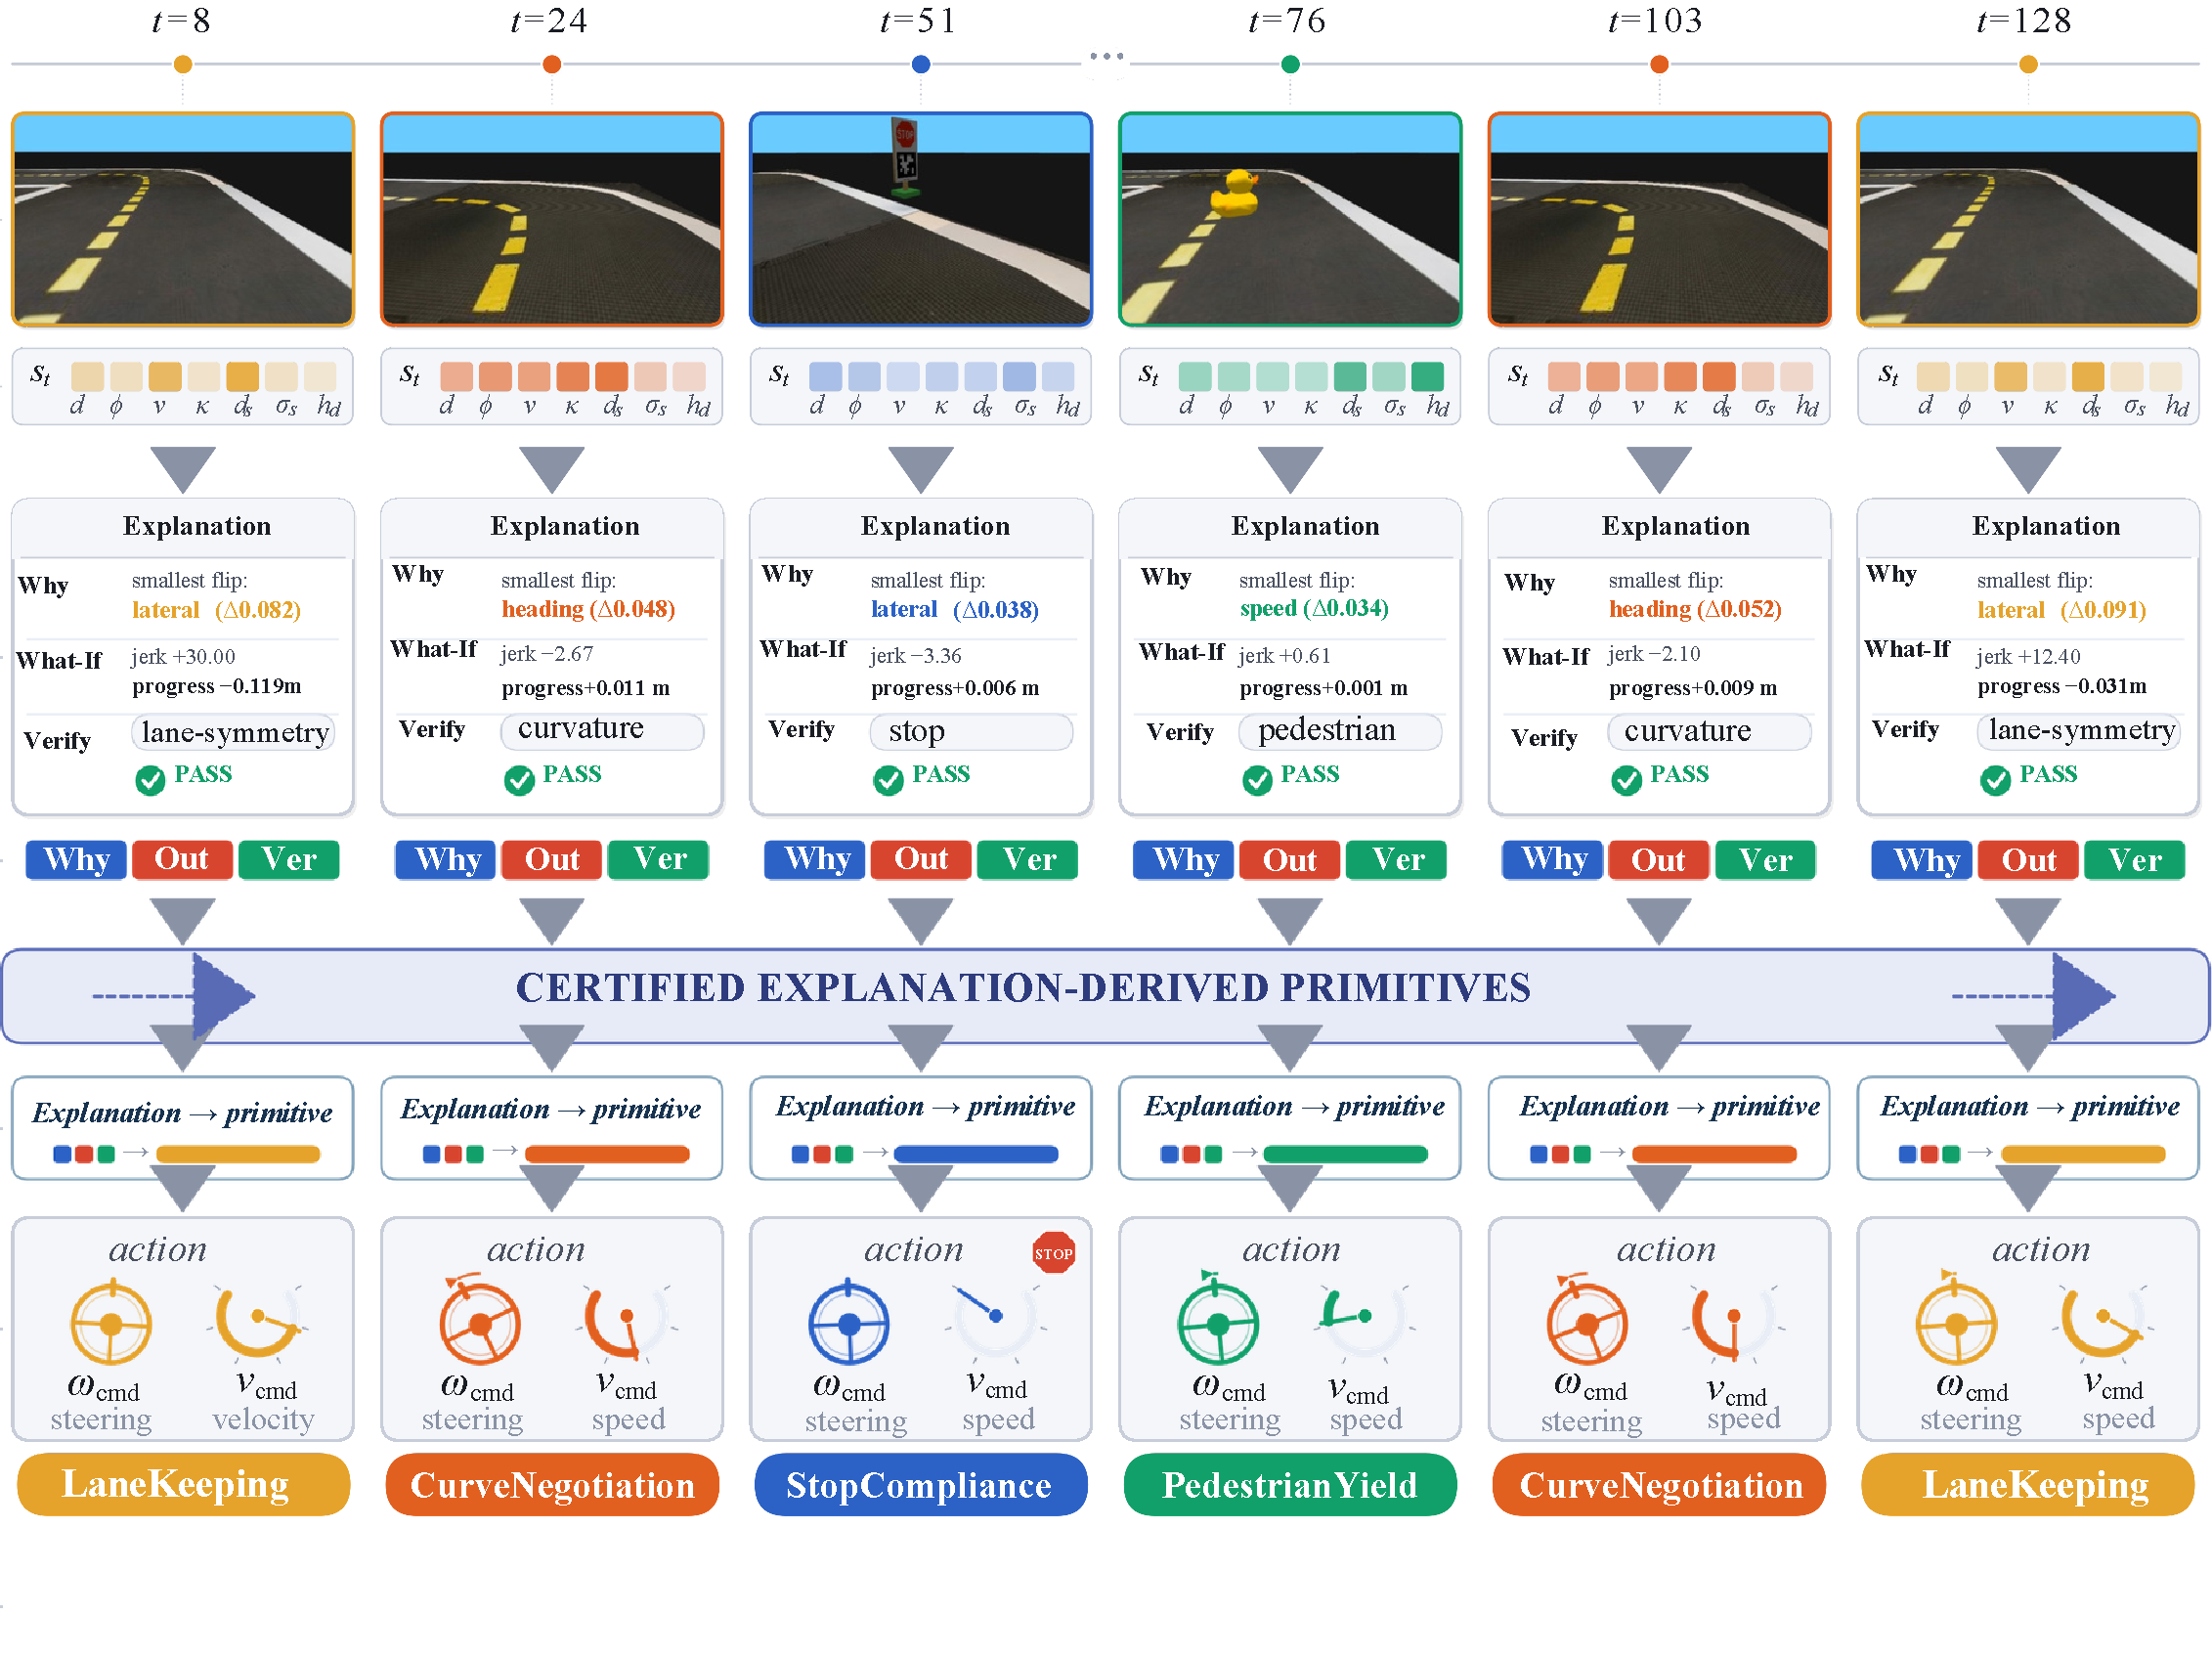
\includegraphics[height=0.40\textheight,keepaspectratio]{mdp_explain.pdf}}\end{center}
\vspace{0.02cm}
\begin{itemize}\setlength{\itemsep}{0.16em}\small
  \item MDP formulation of Duckietown driving; explanations in three pillars:
        \gnum{why this action} $\cdot$ \gnum{what if another} $\cdot$
        \gnum{is it consistent}
  \item Counterfactual rollouts share exogenous noise --- outcome claims are
        settled \gnum{exactly}, across Q-learning, SARSA, SAC, TD3
\end{itemize}
\vspace{0.10cm}
{\color{gold}\bfseries\small github.com/PannnTastic/DuckieMDP \quad
{\color{mintdim}\mdseries$\cdot$ arXiv preprint}\par}
\end{frame}

% ---- 6 · side project: Duckietown.jl ------------------------------------------------
\begin{frame}
\slidehead{Side project --- Duckietown.jl}{The simulator, reborn in Julia}
\begin{columns}[T]
\begin{column}{0.52\textwidth}
\begin{center}\setlength{\fboxsep}{4pt}\colorbox{white}{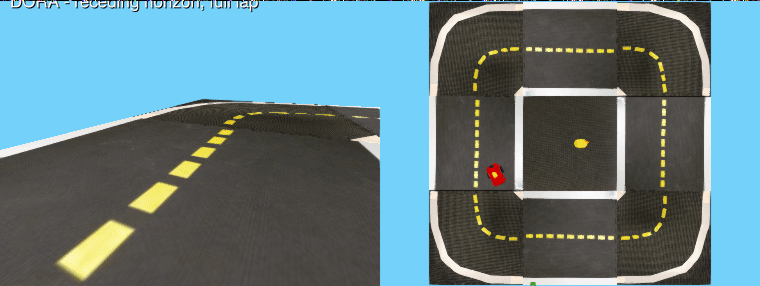
\includegraphics[width=\linewidth]{duckietown_jl.png}}\end{center}
{\color{mintdim}\fontsize{6.5}{8}\selectfont\centering DORA solver completing
a lap, drawn by the package's native renderer\par}
\end{column}
\begin{column}{0.46\textwidth}
\begin{itemize}\setlength{\itemsep}{0.38em}\small
  \item Native \gnum{POMDPs.jl} reimplementation of the DuckieMDP environment
  \item Validated \gnum{decision by decision} against Python --- exact NumPy
        RNG streams, seeded episodes reproduce \gnum{bit for bit}
  \item Native renderer; DORASolvers.jl case study drives a full lap
\end{itemize}
\vspace{0.15cm}
{\color{gold}\bfseries\small github.com/ai-vnv/Duckietown.jl\par}
\end{column}
\end{columns}
\end{frame}

% ==== ACT II — MAIN PROJECT ====================================================

% ---- 7 · divider -----------------------------------------------------------------
\begin{frame}[plain]
\begin{center}
\vspace{1.5cm}
\kicker{Main project --- submitted to IEEE OJ-ITS}
\vspace{0.4cm}

{\poppinsbold\color{white}\fontsize{20}{25}\selectfont
A \textcolor{gold}{Closed-Loop} Evaluation of\\
Capability \textcolor{gold}{Loss and Recovery}\\
in Compressed Driving Policies\par}
\vspace{0.55cm}
{\color{mintdim}\small From learning POMDPs to using one as a research
instrument.\par}
\end{center}
\end{frame}

% ---- 8 · problem ---------------------------------------------------------------
\begin{frame}
\slidehead{The problem}{A policy can pass the benchmark and fail to stop}
\begin{itemize}\setlength{\itemsep}{0.42em}
  \item Learned driving policies run on embedded computers
  \item Standard practice: prune, distill, quantize before deployment
  \item Progress measured by size, latency, aggregate accuracy
  \item Aggregate scores hide \gnum{which behaviors} compression removes
\end{itemize}
\vspace{0.35cm}
{\color{mintdim}\small The question is not only how small the network can get
--- but which learned capabilities survive each stage.\par}
\end{frame}

% ---- 9 · key idea ----------------------------------------------------------------
\begin{frame}
\slidehead{Key idea}{Closed loop, stage by stage — reversed}
\begin{itemize}\setlength{\itemsep}{0.40em}
  \item A policy acts on its own observations: small action drift
        \gnum{compounds} through the feedback loop
  \item Static test-set scores cannot see this
  \item Scenario-based assessment, reversed: \gnum{fix the scenarios and
        seeds}, vary the system under test
  \item Every compression stage is a new configuration to re-certify;
        acceptance criteria fixed \gnum{before} any result
\end{itemize}
\vspace{0.30cm}
{\color{mintdim}\small Four questions: where does driving break $\cdot$ is it
recoverable $\cdot$ does the data decide $\cdot$ does recovery survive lower
precision.\par}
\end{frame}

% ---- 10 · task ---------------------------------------------------------------------
\begin{frame}
\slidehead{The driving task}{Five curricula, shared seeds, rising difficulty}
\whitecard[0.97\linewidth]{fig_task.pdf}
\vspace{0.1cm}
\begin{itemize}\setlength{\itemsep}{0.22em}
  \item C0--C1 lane following $\cdot$ C2 crossing pedestrian $\cdot$ C3 stop
        sign $\cdot$ C4 both
  \item The stop curricula demand interrupting the drive, then re-establishing it
\end{itemize}
\end{frame}

% ---- 11 · system under test ---------------------------------------------------------
\begin{frame}
\slidehead{System under test}{A belief-state visuomotor policy (POMDP + PPO)}
\begin{columns}[T]
\begin{column}{0.56\textwidth}
\whitecard[\linewidth]{fig_pipeline.pdf}
\end{column}
\begin{column}{0.42\textwidth}
\begin{itemize}\setlength{\itemsep}{0.38em}
  \item Camera $\rightarrow$ \gnum{YOLO11n} (objects) $+$ \gnum{MobileNetV3} (lane pose)
  \item EKFs fuse detections over time into a \gnum{29-d belief} vector
  \item Belief-PPO actor: \gnum{73{,}986} parameters (FP32)
  \item Only the actor is compressed; perception stays fixed
\end{itemize}
\end{column}
\end{columns}
\end{frame}

% ---- 12 · how the pipeline works ----------------------------------------------------
\begin{frame}
\slidehead{How the pipeline works}{Ten configurations, one shared ancestry}
\begin{itemize}\setlength{\itemsep}{0.30em}
  \item \gnum{A0} original actor (reference)
  \item \gnum{A1} structured pruning, hidden width 256 $\rightarrow$ 64
  \item \gnum{A2} $+$ distillation on the hardest curriculum only
  \item \gnum{A3} $+$ distillation on balanced C0--C4 data (62{,}176 states)
  \item \gnum{A6} A3 $\rightarrow$ post-training INT8 \quad
        \gnum{A8} A3 parent $\rightarrow$ QAT INT8
  \item \gnum{A9} A3 $\rightarrow$ FP16 cast (precision control)
  \item \gnum{A4, A5, A7} controls: unpruned INT8, no-distill INT8, historical QAT
\end{itemize}
\vspace{0.22cm}
{\color{mintdim}\small Every arrow is evaluated the same way --- no configuration
is trusted on the previous stage's evidence.\par}
\end{frame}

% ---- 13 · protocol --------------------------------------------------------------------
\begin{frame}
\slidehead{Evaluation protocol}{400 matched episodes, two independent axes}
\begin{itemize}\setlength{\itemsep}{0.40em}
  \item \gnum{10 models $\times$ 5 curricula $\times$ 8 seeds} --- identical seeds for all
  \item Acceptance checks preregistered: completion, progress, collisions,
        stop compliance and restart, lane keeping, clearance
  \item Evaluation backend verified \gnum{bit-for-bit} reproducible
  \item Axis 1: task verdicts (does it drive?)
  \item Axis 2: action fidelity vs.\ the original on identical inputs (does it imitate?)
\end{itemize}
\end{frame}

% ---- 14 · findings 1+2 ----------------------------------------------------------------
\begin{frame}
\slidehead{Findings 1 \& 2}{Pruning breaks driving; rehearsal decides recovery}
\begin{itemize}\setlength{\itemsep}{0.42em}
  \item Structured pruning: 73{,}986 $\rightarrow$ \gnum{6{,}210} parameters
        ($-$91.6\%) --- \gnum{fails all five} curricula
  \item Same teacher, loss, optimizer, budget --- only the rehearsal data differs
  \item Distill on the hardest curriculum only $\rightarrow$ recovers \gnum{C3--C4 only}
  \item Balanced rehearsal across all five $\rightarrow$ recovers \gnum{all five}
\end{itemize}
\vspace{0.35cm}
{\color{mintdim}\small What the student rehearses is what the student keeps.\par}
\end{frame}

% ---- 15 · finding 3 --------------------------------------------------------------------
\begin{frame}
\slidehead{Finding 3}{INT8 undoes a completed recovery}
\begin{center}\setlength{\fboxsep}{5pt}\colorbox{white}{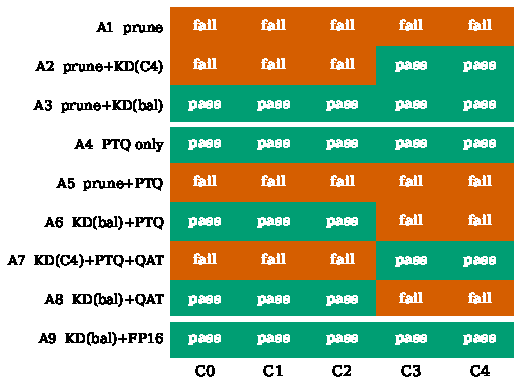
\includegraphics[height=0.56\textheight,keepaspectratio]{fig_matrix.pdf}}\end{center}
\vspace{0.04cm}
\begin{itemize}\setlength{\itemsep}{0.14em}\small
  \item Both INT8 routes fail C3--C4 from one byte-identical checkpoint
  \item Stop-task completion falls from \gnum{8/8 to 3/8} under PTQ
\end{itemize}
\end{frame}

% ---- 16 · phenotypes -------------------------------------------------------------------
\begin{frame}
\slidehead{Opposite failure phenotypes}{One checkpoint, two ways to fail a stop}
\begin{columns}[T]
\begin{column}{0.52\textwidth}
\begin{center}\setlength{\fboxsep}{4pt}\colorbox{white}{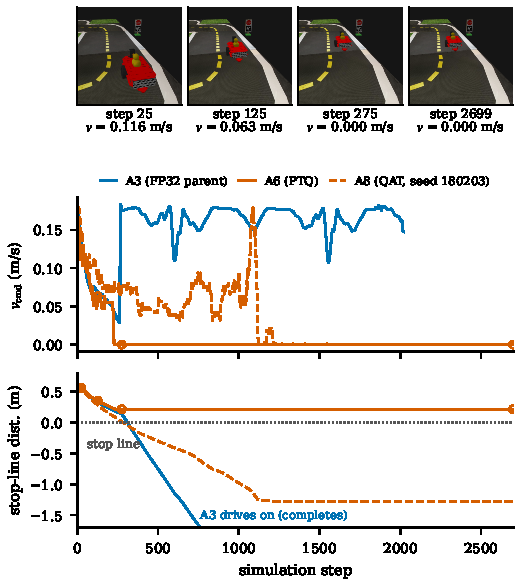
\includegraphics[height=0.74\textheight,keepaspectratio]{fig_stop.pdf}}\end{center}
\end{column}
\begin{column}{0.46\textwidth}
\begin{itemize}\setlength{\itemsep}{0.40em}
  \item \gnum{A6 (PTQ)} brakes correctly, parks \gnum{0.22 m} before the line
        --- and never moves again (to the 2700-step horizon)
  \item \gnum{A8 (QAT)} drives \gnum{through} the stop at low speed while the
        stop is still required
  \item Same parent, same task, opposite failures
\end{itemize}
\end{column}
\end{columns}
\end{frame}

% ---- 17 · findings 4+5 -----------------------------------------------------------------
\begin{frame}
\slidehead{Findings 4 \& 5}{Controls and fidelity: the cause is the interaction}
\begin{itemize}\setlength{\itemsep}{0.42em}
  \item Same PTQ on the \gnum{unpruned} actor $\rightarrow$ passes all five
  \item \gnum{FP16 cast} of the recovered actor $\rightarrow$ keeps all five
  \item So the failure is \gnum{narrow width $\times$ INT8}, not precision alone
  \item QAT imitates the original \gnum{more closely} than PTQ --- and drives worse
  \item The unpruned INT8 control drives everything --- and fails the
        similarity thresholds
\end{itemize}
\vspace{0.25cm}
{\color{mintdim}\small Action-level similarity is not an acceptance test ---
in either direction.\par}
\end{frame}

% ---- 18 · cost ------------------------------------------------------------------------
\begin{frame}
\slidehead{What compression buys}{Actor cost across precisions}
\vspace{0.1cm}
\begin{center}
{\color{mint}
\begin{tabular}{lccc}
\toprule
 & \textcolor{white}{\bfseries Param.\ memory} &
   \textcolor{white}{\bfseries Median latency} &
   \textcolor{white}{\bfseries All curricula} \\
\midrule
A3 FP32 & 24.8 KB & 19.4 $\mu$s & \textcolor{gold}{pass} \\
A9 FP16 & \gnum{12.4 KB} & 24.5 $\mu$s ($+$26\%) & \textcolor{gold}{pass} \\
A6 INT8 & \gnum{7.6 KB} & \gnum{12.9 $\mu$s} (1.50$\times$) & fail C3--C4 \\
\bottomrule
\end{tabular}\par}
\end{center}
\vspace{0.25cm}
\begin{itemize}\setlength{\itemsep}{0.24em}
  \item FP16 halves memory but is slower here (no native half path on this CPU)
  \item The actor is under \gnum{0.1\%} of end-to-end step cost --- perception dominates
\end{itemize}
\end{frame}

% ---- 19 · takeaways --------------------------------------------------------------------
\begin{frame}
\slidehead{Takeaways}{Judge compressed policies by how they drive}
\begin{itemize}\setlength{\itemsep}{0.44em}
  \item Compression is a sequence of \gnum{behavioral transitions}: lose,
        recover, lose again
  \item Evaluate \gnum{every stage} in closed loop --- no stage is safe by inheritance
  \item Choose rehearsal data to cover \gnum{everything} the policy must keep
  \item A completed recovery is \gnum{not} robust to a later precision cut
  \item Action-level similarity is not an acceptance test
\end{itemize}
\end{frame}

% ---- 20 · future works -----------------------------------------------------------------
\begin{frame}
\slidehead{Future works}{Where this goes next}
\begin{itemize}\setlength{\itemsep}{0.42em}
  \item \gnum{Wider settings}: more quantization configurations, more training
        realizations, more seeds
  \item \gnum{Compress perception}: the other 99.9\% of step cost, under the
        same acceptance protocol
  \item \gnum{Transfer the protocol}: other policy stacks, other simulators,
        eventually hardware
  \item \gnum{Julia-native line}: Duckietown.jl as the ground for solver-level
        V\&V experiments
\end{itemize}
\end{frame}

% ==== ACT III — CLOSING ========================================================

% ---- 21 · reflection -------------------------------------------------------------------
\begin{frame}
\slidehead{What the internship built}{Fundamentals first, then honest evaluation}
\begin{itemize}\setlength{\itemsep}{0.44em}
  \item From backend engineering to an \gnum{RL / POMDP research workflow}
  \item \gnum{4 public repos} $\cdot$ \gnum{2 papers} $\cdot$ \gnum{1 Julia
        package}
  \item From a bad first month to an \gnum{OJ-ITS submission}
  \item The lesson that stuck: measure what matters, \gnum{in closed loop}
\end{itemize}
\end{frame}

% ---- 22 · thanks -----------------------------------------------------------------------
\begin{frame}[plain]
\begin{center}
\vspace{1.1cm}
\kicker{Thank you}
\vspace{0.3cm}

{\poppinsbold\color{white}\fontsize{20}{24}\selectfont
Questions?\par}
\vspace{0.5cm}
{\color{mint}\small Everything in this talk is public:\par}
\vspace{0.15cm}
{\color{gold}\bfseries\small
github.com/ai-vnv/CompressedAutoDriving \quad $\cdot$ \quad
github.com/PannnTastic/DuckieMDP\par}
\vspace{0.08cm}
{\color{gold}\bfseries\small
github.com/PannnTastic/Decision-Making-Under-Uncertainty \quad $\cdot$ \quad
github.com/ai-vnv/Duckietown.jl\par}
\vspace{0.55cm}
{\color{mintdim}\fontsize{7}{9}\selectfont
Internship summary --- AI Verification \& Validation Lab\par}
\end{center}
\end{frame}

\end{document}
